% ----------------------------------------
% Chap: Literaturforschung
% ----------------------------------------
\chapter{Literaturforschung der experimentellen Techniken zur Schmierfilmdickenmessung in EHD-Kontakten}
\label{chap:literaturforschung_der_experimentellen_technik_in_ehd_schmierung}

% ----------------------------------------
% Sec: Optische Messmethoden
% ----------------------------------------
\section{Optische Messung der EHD Schmierfilmdicke}
\label{sec:optische_messung_der_ehd_schmierfilmdicke}

% ----------------------------------------
% Sub: Lichtinterferenz
% ----------------------------------------
\subsection{Licht Interferometrie}
\label{ssec:licht_interferometrie}

% ----------------------------------------
% Sub: Variante Methoden von Lichtinterferenz
% ----------------------------------------
\subsection{Variante von der klassichen optischen Interferometrie Methode}
\label{ssec:variante_interferometrie}

% ----------------------------------------
% Sec: Elektrische Methode
% ----------------------------------------
\section{Elektrische Messung der EHD Schmierfilmdicke}
\label{sec:elektrische_messung_der_ehd_schmierfilmdicke}

Neben der optischen Messmethoden gibt es noch die elektrische Messmethode zur Untersuchung der EHD-Schmierung, wie zum Beispiel Widerstand, Kapazität, Entladespannung.
Der Vorteil dieser Methode ist, dass sie direkt bei Maschinenelementen, welche aus Stahl sind, während Betrieb verwendet werden kann.
Allerdings gibt es auch Nachteile.
Die Form des Kontakts, wo die große lokale Verformung stattfindet, ist nur vermutet und stark vereinfacht.
Die hat den Einfluss auf die Widerstand-,Kapazität-Messergebnisse.
Ein Faktor noch ist die Sauberkeit des Schmierstoffes, welche schwer zu kontrollieren ist.
Generell liefern die elektrische Methode nur die mittlere Werte über den Kontaktbereich und gibt leider keine direkte Indikation der Form des Schmierfilms.

Normalerweise werden die elektrische Methoden für folgende Anwendungen verwendet:
\begin{itemize}
    \item Schmierfilmdickenmessung bei bekannten Schmierstoffen
    \item Detektion des Voll-Schmierfilaufbaus im Kontakt der rauhen Öberflächen
    \item Evaluierung des geschmierten Kontakts unter Einfluss des elektrischen Felds
\end{itemize}

% ----------------------------------------
% Sub: Widerstandmessung
% ----------------------------------------
\subsection{Widerstandmessung}
\label{sub:wiederstandmessung}

Die Widerstandmessmethode ist geeignet, um den Schmierungszustand qualitativ zu beschreiben.
Der Widerstand ist eine Indikation der direkten Berührung der Rauheitspitzen der Kontaktpartner.
Bei vollständiger Oberflächentrennung (Flüssigkeitschmierung) soll der Widerstand in theoretisch unendlich groß sein.
Zum besseren Verständnis der elektrischen Vorgängen im EHD-Kontakt wurde eine Reihe Arbeiten an unterschiedlichen Modellprüfständen und Maschinenelementen durchgeführt.

In einem System bestehend aus einer feststehenden Kugel und einem rotierenden Zylinder hat \textit{Furey} \cite{furey_1961} das Verhalten des elektrischen Widerstands untersucht.
Die Ergebnisse (Abbildung \ref{fig:resistance_vs_time_furey}) zeigten eine große Streuung des Widerstands bei Mischreibung.
Zum Beschreiben für einen isolierenden Schmierfilm definiert er einen Wert von 10$k\Omega$.
In Oszilloskop erkannt er, dass es zwei Zustände des Kontaktwiderstands gabt, hoch und niedrig.
Das zeitliche Verhältnis zwischen den beiden Zuständen wird über Intervalle von 10 $ms$ aufgenommen, ausgewertet und das Ergebnis als prozentualer Anteil des direkten Kontakt angegeben.
Mit dieser Methode konnte er berechnen, wie groß der Anteil der Festkörperkontakte in jedem Reibungszustand ist.
% ----------------------------------------
% Fig: Widerstand - Zeit Furey
% ----------------------------------------
\begin{figure}[htb]
    \centering
    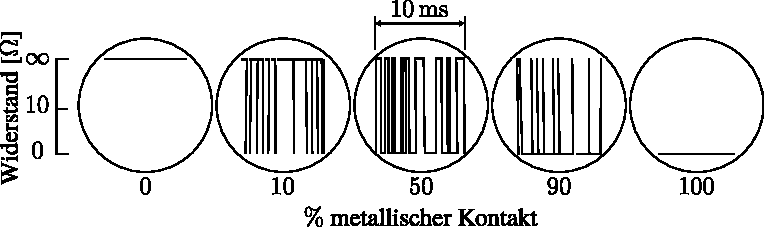
\includegraphics[]{./images/resistance_vs_time_furey.pdf}
    \caption{Der prozentuale Anteil von metallischen Kontakt \cite{furey_1961}}
    \label{fig:resistance_vs_time_furey}
\end{figure}
%

In seiner Arbeit \cite{kuhlmann_2009} verwendete \textit{Kuhlmann} zwei unterschiedliche Systeme zur Widerstandmessung.
Ein System basiert auf die \textit{Wheatstonsche} Brückenschaltung (Abbildung \ref{fig:ersatzschaltbild_messsysteme_kuhlmann} links), welche zur Vermeidung eines Tunneleffektes mit Wechselstrom gespeist wird.
Der Zusammenhang zwischen dem Widerstand $R_L$ des Lagers und der gemessenen Brückenspannung $U_m$ wird durch eine aufwändige Kalibration über variable Referenzwiderstände hergestellt.
Zur Vereinfachung der Messkettenkalibrierung und zur Verbesserung der Messempfindlichkeit bei $R_L$ mehr als 1 $k\Omega$ setzte \textit{Kuhlmann} ein direkt messendes Trägerfrequenz-Messsystem ein (Abbildung \ref{fig:ersatzschaltbild_messsysteme_kuhlmann} rechts).
Der Widerstandszwei wird an einer hochgenauen Wechselstromquelle ($1 \pm 0,2 mA$) angeschlossen.
Aus dem Spannungsabfall über den Gesamtwiderstand ($R_V$ und $R_P$ sind bekannt) konnte er den Lagerwiderstand bestimmen.
% ----------------------------------------
% Fig: Kuhlmann Messsysteme
% ----------------------------------------
\begin{figure}[htb]
    \centering
    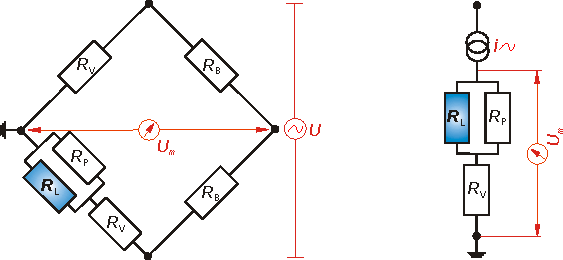
\includegraphics[]{./images/ersatzschaltbild_kuhlmann.pdf}
    \caption{Ersatzschaltbild für die Messsysteme \cite{kuhlmann_2009}}
    \label{fig:ersatzschaltbild_messsysteme_kuhlmann}
\end{figure}
%

Beide obengenannte Messsysteme wurden von \textit{Kuhlmann} bei Fettuntersuchung mit Schrägkugellagern und Kegelrollenlagern bei niedrigen Betriebstemperatur eingesetzt (Abbildung \ref{fig:schema_schraerikula_kerola_kuhlmann}).
Durch eine 0,4 mm dicke Keramikbeschicht zwischen der Lagersitze und der Welle konnte er den Widerstand für beide Lager separat messen.
Abbildung \ref{fig:schema_schraerikula_kerola_kuhlmann} zeigt die elektrische Ersatzschaltbilder für einen Wälzkörper im Schrägkugellager und Kegelrollenlager.
Alle Wälzkörper eines Lagers sind elektrisch parallel geschaltet und der Kontakt zwischen Rollenstirn und Bord beim Kegelrollenlager muss berücksichtigt werden.
% ----------------------------------------
% Fig: Kuhlmann Test Lager
% ----------------------------------------
\begin{figure}[htb]
    \centering
    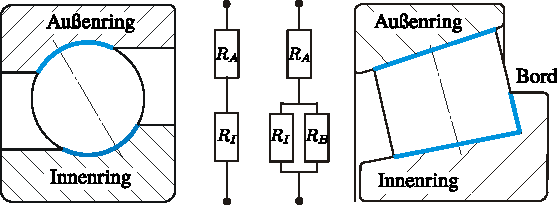
\includegraphics[]{./images/schema_schraegrikula_kerola_kuhlmann.pdf}
    \caption{Schema des Schrägkugellager- und Kegelrollenlager-Einzelkontaktes \cite{kuhlmann_2009}}
    \label{fig:schema_schraerikula_kerola_kuhlmann}
\end{figure}
%

% ----------------------------------------
% Sub: Kapazitätmessung
% ----------------------------------------
\subsection{Kapazitätmessung}
\label{sub:kapazitatmessung}

Der Vorteil bei der Kapazitätmessung ist wie bei der Widerstandsmessung die einfache Anwendung im Maschinenelement.
Es ist auch möglich bei dieser Methode quantitative Schmierfilmdickenmessung durchzuführen, welche bei resistiver Methode schwer oder unmöglich ist.

Auf Basis der Konstantstromladung hat \textit{Barz} \cite{barz_1996} ein System zur kapazitiven Schmierfilmdickenmessung im Wälzlager entwickelt.
Hier werden die Oberflächen zwischen Wälzkörpern, Außenring und Innenring bei einem trennenden Schmierfilm als Kondensator betrachtet.
Die Kapazität des einzelnen EHD-Kontaktes wird nach dem Modell von \textit{Brüser} \cite{brueser_1972} beschrieben.
% ----------------------------------------
% Fig: Brüser Modell des EHD-Kontaktes
% ----------------------------------------
\begin{figure}[htb]
    \centering
    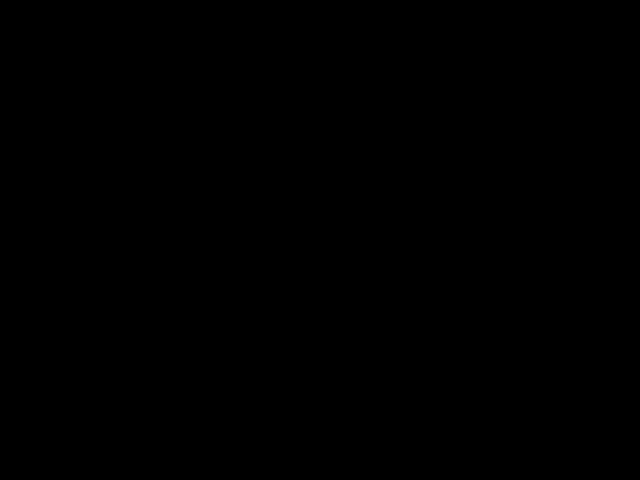
\includegraphics[width=4cm]{./images/blank_img.jpg}
    \caption{Kapazitives Modell eines EHD-Kontaktes \cite{barz_1996}}
    \label{fig:kapazitives_modell_eines_ehd_kontaktes}
\end{figure}
%

Im Modell von \textit{Barz} wird der EHD-Kontakt in drei Bereiche \textit{Einlaufbereich}, \textit{Hertzscher Kontaktbereich} und \textit{Auslaufbereich} geteilt und unter folgenden Annahmen betrachtet:
%
\begin{enumerate}
    \item Der Einlaufbereich ist vollständig mit Schmierstoff gefüllt
    \item Im Hertzschen Kontaktbereich herrscht es eine konstante Schmierfilmdicke $h_0$
    \item Die Einschnürung vor dem Auslaufbereich wird vernachlässigt
    \item Im Auslaufbereich haftet der Schmierstoff gleichmäßig an den Kontaktpartner an
    \item Das elektrische Feld im Hertzschen Bereich ist homogen
\end{enumerate}
%

Mit dieser Annahmen kann man die Kontaktkapazität so berechnen:
%
\begin{equation}
    C_K = C_{Einlauf} + C_{Hertz} + C_{Auslauf}
    \label{eq:kontaktkapazitaet}
\end{equation}
%
Aufgrund dem großen Einfluss und der linearen Proportional von der $C_{Hertz}$ mit der $C_K$ vereinfachte \textit{Barz} die Kontaktkapazität als:
%
\begin{align}
    C_K = f(C_{Hertz}) = k_C C_{Hertz} \\
    C_{Hertz} = \varepsilon_0 \varepsilon_r \cfrac{A_{Hertz}}{h_0}
    \label{eq:kontaktkapazitaet_vereinfach}
\end{align}
%
\textit{Barz} definierte einen Umrechnungsfaktor $k_C$ in der Gleichung \ref{eq:kontaktkapazitaet_vereinfach}, welcher die $C_{Einlauf}$ und die $C_{Auslauf}$ berücksichtigt.
Der Umrechnungsfaktor ist von den Betriebsbedingungen, dem Lager, dem Schmierstoff, der Laufzeit etc. abhängig.
Selbst ist er von der Schmierfilmdicke abhängig, da das Verhältnis zwischen $C_{Einlauf}$ und $C_{Auslauf}$ bei der Änderung der Schmierfilmdicke nicht konstant bleibt.
Für den betrachten Fall mit axial belasteten Spindellagern hat \textit{Barz} mit dem Wert $k_C = 3,5$ bestimmt.

Da die Kontakte zwischen den Wälzkörpern mit dem Außenring und dem Innenring nicht gleich sind, führte \textit{Barz} weiterhin einen Faktor $k_h$ zur individuellen Bestimmung der Schmierfilmdicke an der beiden Ringen ein.
Der ist das Verhältnis von den nach EHD-Theorie berechneten Schmierfilmdicken am Innenring $h_{EHD,i}$ und am Außenring $h_{EHD,a}$ und berechnet sich unter einer Annahme, dass die Schmierungbedingungen am Innenring und Außenring gleich sind, zu
%
\begin{equation}
    k_h = \cfrac{h_a}{h_i} = \cfrac{h_{mess,a}}{h_{mess,i}} = \cfrac{h_{EHD,a}}{h_{EHD,i}}
    \label{eq:kh_faktor}
\end{equation}
%
Schließlich berechnen sich die Schmierfilmdicken am Innenring bzw. am Außenring zu
%
\begin{align}
    h_{mess,i} = 2 Z k_C \varepsilon_0 
                \cfrac{(\varepsilon_{r,i} A_{Hertz,i}) \left( \varepsilon_{r,a} \cfrac{A_{Hertz,a}}{k_h} \right) }
                      {(\varepsilon_{r,i} A_{Hertz,i}) + \left( \varepsilon_{r,a} \cfrac{A_{Hertz,a}}{k_h} \right) }
                \cfrac{1}{C_{ges}}
    \label{eq:schmierfilmdicke_am_innenring}
\end{align}
%


% ----------------------------------------
% Sec: Alternative Methoden
% ----------------------------------------
\section{Alternative EHD Schmierfilmdicke Messmethoden}
\label{sec:alternative_messmethoden}

% ----------------------------------------
% Sub: Taktile Messung
% ----------------------------------------
\subsection{Taktile}
\label{sub:taktil}

% ----------------------------------------
% Sub: Ultrashall Messung
% ----------------------------------------
\subsection{Ultraschall}
\label{sub:ultraschall}

% ----------------------------------------
% Sub: Laserinduzierte Messung
% ----------------------------------------
\subsection{Laserinduzierte Fluoreszenz}
\label{sub:laserinduzierte_fluoreszenz}
